\section{Ovládání západky a IR komunikace}
\addcontentsline{toc}{section}{Ovládání západky a IR komunikace}

\begin{figure}[htbp]
    \centering
    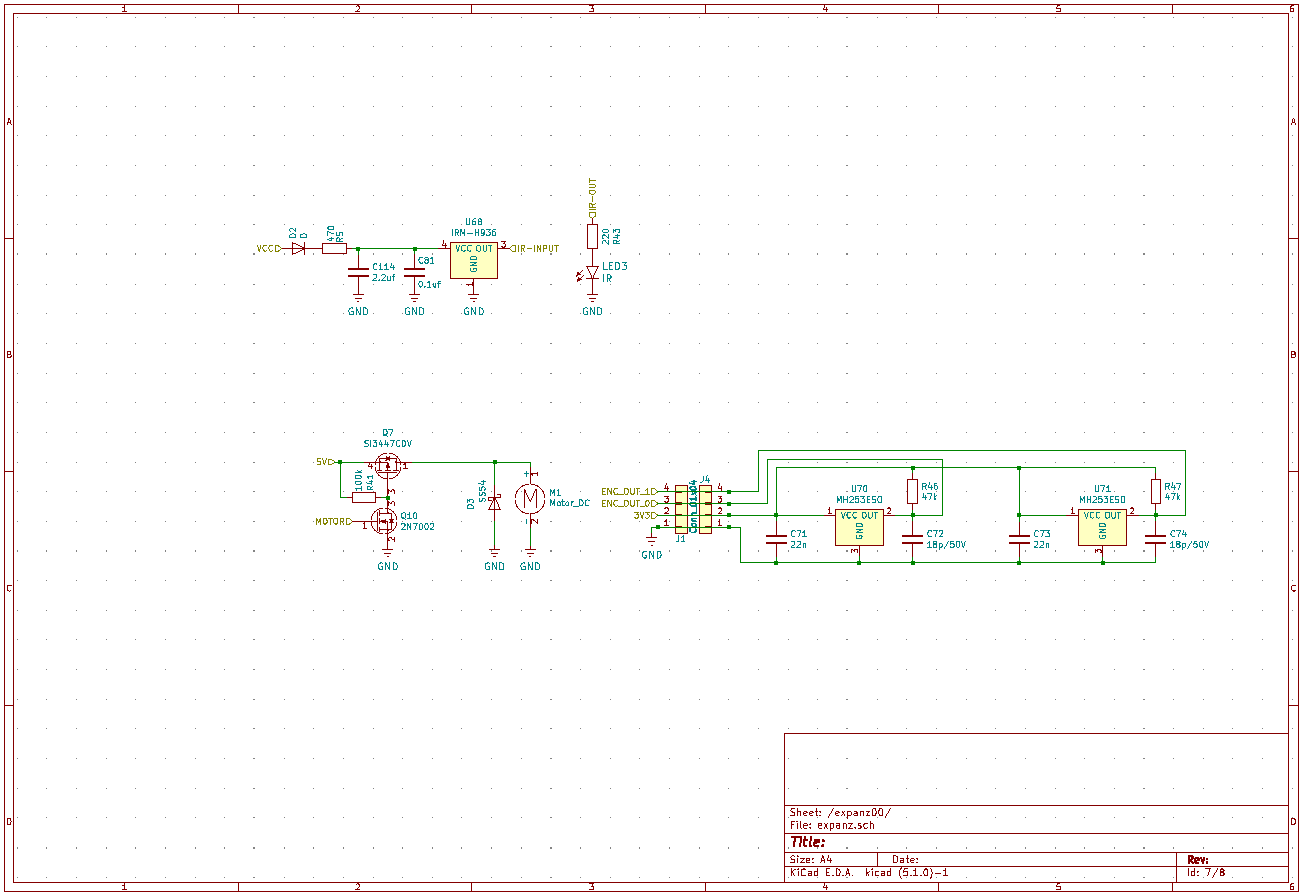
\includegraphics[width=\textwidth]{kapitoly/obrazky/E4/ir_motor_enkoder/sch.png}
    \caption{zapojení řízení motoru, enkoderu a IR komunikace}
    \label{fig:E4-ir-motor-enkoder}
\end{figure}

\newpage

\paragraph{IR komunikace}
\addcontentsline{toc}{paragraph}{IR komunikace}
IR slouží primárně pro identifikaci dveří, při vkládání většího množství dveří do stejného trezoru.
Trezor totiž počítá s možností vkládání více dveří do jednoho trezoru, což je jedna ze schopností, která slouží více trezoru jako hračce a ne trezoru jako bezpečnostní schránce.
Tento trezor s více otvory by zároveň mohl sloužit jako jakýsi displej a na to potřebuje vědět které dveře jsou kde na což slouží právě IR komunikace.

Jako IR přijímač jsem z nabídky JLCPCB zvolil \href{https://datasheet.lcsc.com/szlcsc/1912111437_Everlight-Elec-IRM-H936-TR2_C264266.pdf}{IRM-H936}. V nabídce JLCPCB jsou v této době jen 
tři IR-přijímače, jeden z nich je THT a~je~namířen rovnoběžně s deskou a z tohoto důvodu nevyhovuje. Druhé dva jsou právě IRM-H936 a \href{https://datasheet.lcsc.com/szlcsc/2010221806_Everlight-Elec-IRM-H638T-TR2-DX_C390031.pdf}{IRM-H638},
z nichž IRM-H936 má skoro poloviční výšku a širší uhel záběru a to byl důvod jeho volby.

Druhou částí IR komunikace je vysílač který je zajištěn jednoduše IR ledkou.

\begin{figure}[htbp]
    \centering
    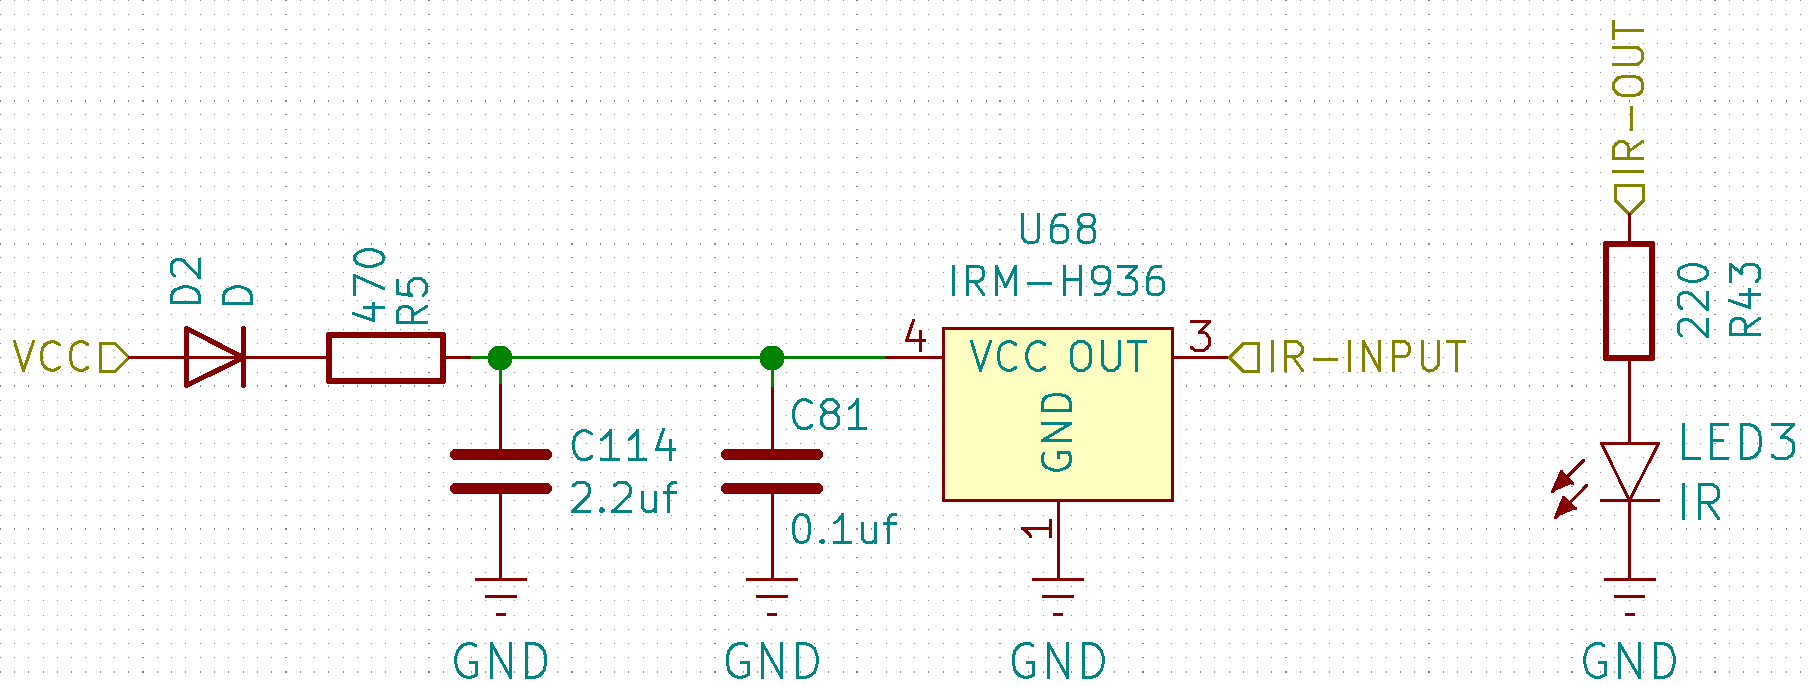
\includegraphics[width=\textwidth]{kapitoly/obrazky/E4/ir_motor_enkoder/IR.png}
    \caption{zapojení IR vysílače a přijímače}
    \label{fig:E4-ir}
\end{figure}

\newpage

\paragraph{Ovládání motoru}
\addcontentsline{toc}{paragraph}{Ovládání motoru}
Protože motor je napájen z 5V větvě a protože ho připínám k napájení a ne k zemi nemůžu ho ovládat přímo z procesoru, proto je Q7 napojen na Q10 který je teprve řízen ESP. 
Kvůli napěťový špičkám které při běhu vznikají na komutátoru motoru je zde i zpětná schottkyho dioda, D3.% D3 skrz sebe propustí záporné napětí, které muže na vzniknout motoru.

\begin{figure}[htbp]
    \centering
    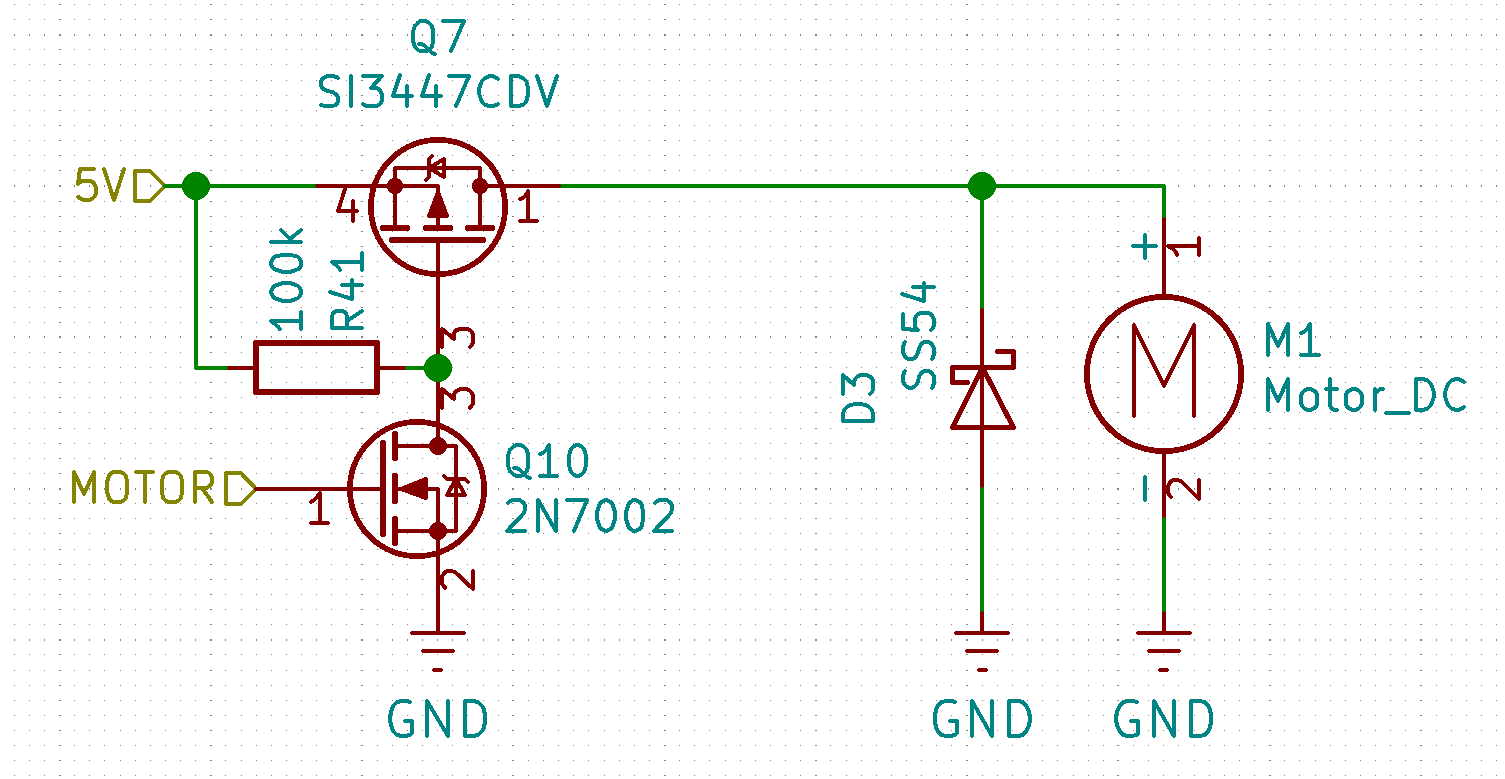
\includegraphics[width=\textwidth]{kapitoly/obrazky/E4/ir_motor_enkoder/ovladani_motoru.png}
    \caption{zapojení řízení motoru}
    \label{fig:E4-motor}
\end{figure}

\newpage

\paragraph{Enkoder}
\addcontentsline{toc}{paragraph}{Enkoder}

\begin{wrapfigure}[13]{R}{0.65\textwidth}
    \centering
    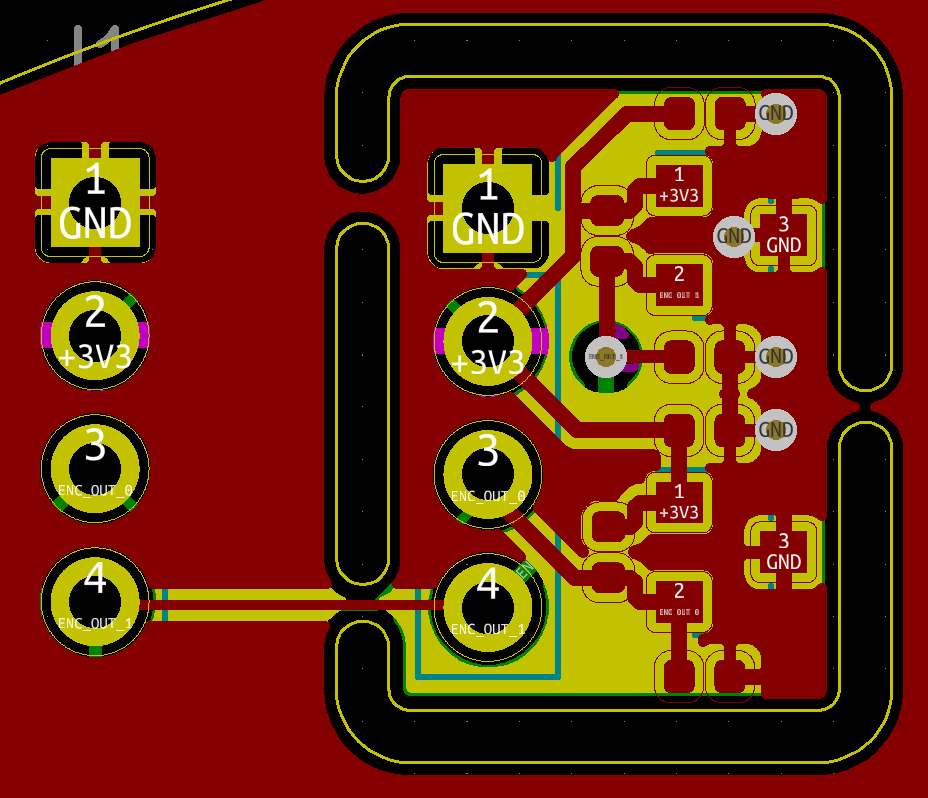
\includegraphics[width= 0.6\textwidth]{kapitoly/obrazky/E4/ir_motor_enkoder/pcb-enc.png}
    \caption{\label{fig:E4-enkoder_pcb}vzhled na desce}
\end{wrapfigure}
Aby bylo možno motor polohovat do správné polohy je nutné mít zpětnou vazbu o~jeho poloze. Vzhledem k~tomu že motor otáčí magnetem, samo se nabízí využít magnetický enkodér. 
Proto jsou na desce dvě digitální hallovi sondy \href{https://datasheet.lcsc.com/szlcsc/Magnesensor-Tech-MST-MH253ESO_C114369.pdf}{MH253ESO}, které se překlopí podle toho v jakém pólu 
se nachází. Protože na desce s~led kruhem by sondy museli být na opačné straně než ledky, takže by se museli pájet ručně protože JLCPCB osazuje jen z~jedné straně. Hlavní deska je ale zase, 
kvůli velikosti baterek, moc daleko od magnetu. Abych tedy nemusel dělat třetí desku jen kvůli enkodéru, zvolil jsem možnost vylomitelného enkodéru. Na hlavní desce jsem tedy nakreslil 
enkodér s konektorem a objel jsem ho frézou aby se dal při montáži trezoru z desky vylomit a posunout do ideální polohy.

\begin{figure}[htbp]
    \centering
    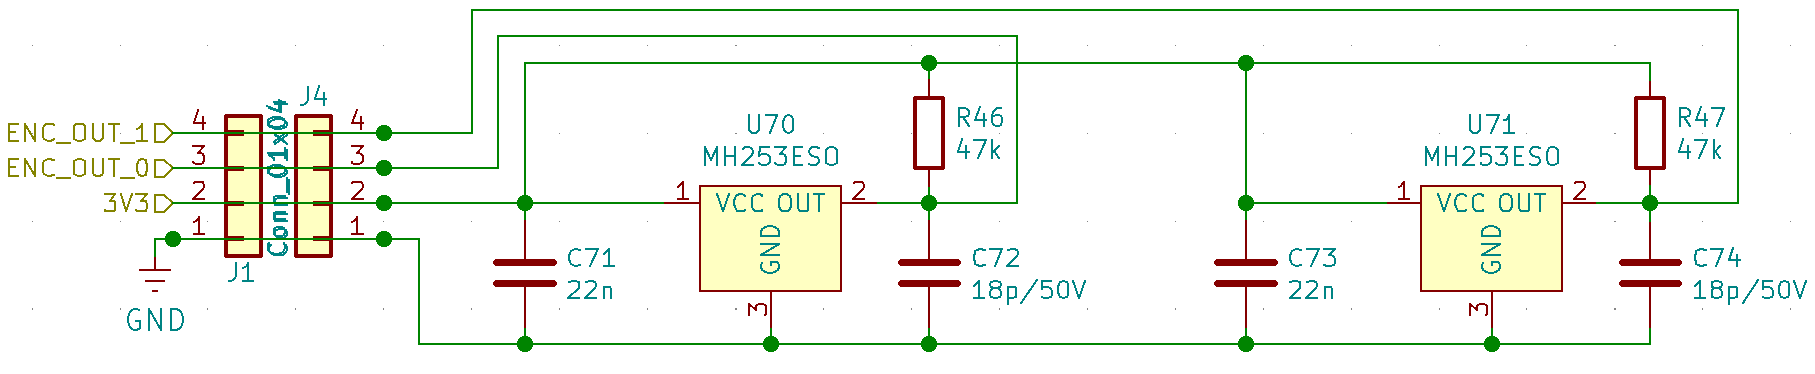
\includegraphics[width=\textwidth]{kapitoly/obrazky/E4/ir_motor_enkoder/enc.png}
    \caption{zapojení enkoderu}
    \label{fig:E4-enkoder}
\end{figure}
